\chapter{信号分析与描述}
\label{chap:signal-analysis}

\begin{focusbox}{本章复习路线}
先理解“时域看变化，频域看组成”，再掌握“周期信号用傅里叶级数，瞬变信号用傅里叶变换”。本章的知识主线是：
\[
\text{强度参数}\ \longrightarrow\ \text{基本变换对}
\ \longrightarrow\ \text{加窗与频移}\ \longrightarrow\ \text{调制频谱}.
\]
\textbf{学习目标：}能判断信号类型，计算强度参数，利用基本变换对和变换性质求频谱，并解释幅频图、相频图及频带重叠现象。
\end{focusbox}

\begin{table}[H]
\centering\small
\begin{tabularx}{\linewidth}{@{}p{3.4cm} X@{}}
\toprule
复习模块 & 核心能力 \\
\midrule
信号强度 & 区分均值、绝对均值、均方值与方均根值，完成周期平均计算。 \\
基本频谱 & 用直接积分求单边指数频谱，并从复数表达式得到幅相谱。 \\
广义变换 & 理解符号、阶跃与冲激的变换，保留主值项和零频冲激项。 \\
加窗与截断 & 用时域乘积和频域卷积解释主瓣、旁瓣与频谱展宽。 \\
衰减振荡 & 用欧拉公式和频移构造复频谱，判断幅值与实际峰位。 \\
调制与采样 & 判断频谱搬移、周期复制及频带重叠的条件。 \\
\bottomrule
\end{tabularx}
\end{table}

\section{信号的分类与描述}

\subsection{确定性、周期性与随机性}

\dfn{确定性信号与随机信号}{确定性信号可用确定的数学关系或规则描述；随机信号的单次波形不能事先准确预测，通常用概率统计方法描述其特征。}

\dfn{周期信号}{若存在 $T_0>0$，使所有适用的 $t$ 均满足
\[
x(t+T_0)=x(t),
\]
则称 $x(t)$ 为周期信号。最小正周期为基本周期，相应基频和基角频率为
\[
f_0=\frac{1}{T_0},\qquad \omega_0=\frac{2\pi}{T_0}=2\pi f_0.
\]}

多个正弦信号相加，只有当各非零频率之间的比值都是有理数时，才存在共同周期。例如 $\sin t+\sin 2t$ 为周期信号，而 $\sin t+\sin(\sqrt{2}\,t)$ 为准周期信号。

\nt{“非周期”并不必然意味着“连续频谱”。准周期信号仍可由离散谱线组成；矩形脉冲等瞬变信号通常具有连续频谱。单边衰减指数在有限时间后趋近于零，但不会严格等于零，因此不属于严格时限信号。}

\subsection{时间与幅值是否连续}

\begin{table}[H]
\centering
\begin{tabularx}{\linewidth}{@{}l X@{}}
\toprule
类别 & 判断依据 \\
\midrule
连续时间信号 $x(t)$ & 时间变量连续；波形可以含跳变，如阶跃。 \\
离散时间信号 $x[n]$ & 时间变量只取离散点，如等间隔采样序列。 \\
模拟信号 & 时间和幅值都连续取值。 \\
数字信号 & 时间离散，幅值经过量化也离散取值。 \\
\bottomrule
\end{tabularx}
\end{table}

采样使时间离散，量化使幅值离散；这两个操作应分别理解。连续时间不等于波形在每个时刻都连续。

\subsection{能量信号、功率信号与时频范围}

\dfn{能量与平均功率}{对实信号或复信号统一使用模平方：
\[
E_x=\int_{-\infty}^{\infty}|x(t)|^2\diff t,
\qquad
P_x=\lim_{L\to\infty}\frac{1}{2L}\int_{-L}^{L}|x(t)|^2\diff t.
\]
$0<E_x<\infty$ 为能量信号，且 $P_x=0$；$0<P_x<\infty$ 为功率信号，且能量无限。零信号及平均功率不存在的情形需单独判断。}

\begin{Example}[breakable=false]{两种典型信号}{}
对 $x(t)=Ae^{-at}u(t)$，$a>0$，
\[
E_x=\int_0^{\infty}|A|^2e^{-2at}\diff t=\frac{|A|^2}{2a},
\]
所以它是能量信号。对 $x(t)=A\sin(\omega_0t)$，$\omega_0>0$，
\[
P_x=\frac{1}{T_0}\int_0^{T_0}A^2\sin^2(\omega_0t)\diff t=\frac{A^2}{2},
\]
所以它是功率信号。两者都可持续无限长，分类依据是积分与极限。
\end{Example}

\textbf{时限信号：}某有限时间区间外恒为零。\quad
\textbf{频限信号：}某有限频率区间外频谱恒为零。非零信号不能同时严格时限且严格频限；有限长度矩形窗有无限延伸的旁瓣。

以 $t=0$ 为起点，$t<0$ 时为零的信号称为单边信号，可记为 $x(t)=g(t)u(t)$。对线性时不变系统，因果性要求冲激响应在 $t<0$ 时为零，即系统不会在输入发生前响应。信号是否单边与时间原点的选取有关，判断系统因果性则应检查其冲激响应。

\clearpage
\subsection{时域与频域各回答什么问题}

时域描述回答“何时发生、幅值如何变化、持续多久”；频域描述回答“含有哪些频率、每种频率有多强、相位如何”。对多频率叠加或受噪声干扰的信号，频域更便于识别成分。

\dfn{欧拉公式}{
\[
e^{\pm\iu\theta}=\cos\theta\pm\iu\sin\theta,\qquad \iu^2=-1,
\]
\[
\cos\theta=\frac{e^{\iu\theta}+e^{-\iu\theta}}{2},\qquad
\sin\theta=\frac{e^{\iu\theta}-e^{-\iu\theta}}{2\iu}.
\]
复指数 $e^{(\sigma+\iu\omega)t}=e^{\sigma t}e^{\iu\omega t}$ 中，$\sigma$ 控制增长或衰减，$\omega$ 控制振荡。}

\section{周期信号与离散频谱}

\subsection{三角形式与复指数形式}

满足狄利克雷充分条件的周期信号可作傅里叶级数展开：一周期内绝对可积、只有有限个极值与有限个第一类间断点。在连续点，级数收敛到函数值；跳变点收敛到左右极限的平均值。

\dfn{三角形式傅里叶级数}{将常数项记为 $a_0$，周期信号展开为：
\[
x(t)=a_0+\sum_{n=1}^{\infty}\bigl[a_n\cos(n\omega_0t)+b_n\sin(n\omega_0t)\bigr],
\]
\begin{align*}
a_0&=\frac{1}{T_0}\int_{t_*}^{t_*+T_0}x(t)\diff t,\\
a_n&=\frac{2}{T_0}\int_{t_*}^{t_*+T_0}x(t)\cos(n\omega_0t)\diff t,\\
b_n&=\frac{2}{T_0}\int_{t_*}^{t_*+T_0}x(t)\sin(n\omega_0t)\diff t.
\end{align*}
积分区间可取任意完整周期。有些教材写 $a_0/2$，对应常数系数会多一倍，不要混用。}

\[
a_n\cos(n\omega_0t)+b_n\sin(n\omega_0t)
=A_n\cos(n\omega_0t-\theta_n),
\]
\[
A_n=\sqrt{a_n^2+b_n^2},\qquad \theta_n=\operatorname{atan2}(b_n,a_n).
\]
若改写为 $A_n\sin(n\omega_0t+\varphi_n)$，则 $\varphi_n=\operatorname{atan2}(a_n,b_n)$。使用双参数反正切以保留象限；当 $A_n=0$ 时，相位无定义。

\dfn{复指数形式傅里叶级数}{
\[
x(t)=\sum_{n=-\infty}^{\infty}C_ne^{\iu n\omega_0t},\qquad
C_n=\frac{1}{T_0}\int_{t_*}^{t_*+T_0}x(t)e^{-\iu n\omega_0t}\diff t.
\]
对实信号，$C_{-n}=C_n^*$，且对于 $n>0$，
\[
C_0=a_0,\quad C_n=\frac{a_n-\iu b_n}{2},\quad
|C_n|=|C_{-n}|=\frac{A_n}{2}.
\]}

\nt{负频率描述复指数在复平面上的相反旋转方向。一个实余弦由正、负频率各一半的复指数构成；三角形式的单边幅值 $A_n$ 与复指数双边幅值 $|C_n|$ 相差两倍（直流分量不加倍）。虚部与相位是不同概念，相位需由实部和虚部共同确定。}

\subsection{谱线、对称性与方波例子}

周期信号具有\textbf{离散性}（只在特定频率有谱线）、\textbf{谐波性}（频率是基频的整数倍）及通常的\textbf{收敛性}（谐波系数随次数增大趋于零，但未必逐项单调减小）。

\ex{正弦、余弦与奇对称方波}{
对 $A\cos(2\pi f_0t)$，$C_1=C_{-1}=A/2$；对 $A\sin(2\pi f_0t)$，$C_1=-\iu A/2$，$C_{-1}=\iu A/2$。

对一周期内 $x(t)=A$（$0<t<T_0/2$）、$x(t)=-A$（$-T_0/2<t<0$）的方波，奇对称使 $a_0=a_n=0$，计算得
\[
b_n=\begin{cases}4A/(n\pi),&n\text{为奇数},\\0,&n\text{为偶数},\end{cases}
\]
\[
x(t)=\frac{4A}{\pi}\left[\sin\omega_0t+\frac{\sin3\omega_0t}{3}
+\frac{\sin5\omega_0t}{5}+\cdots\right].
\]
因此只有奇次谐波，幅值按 $1/n$ 衰减。
\begin{center}
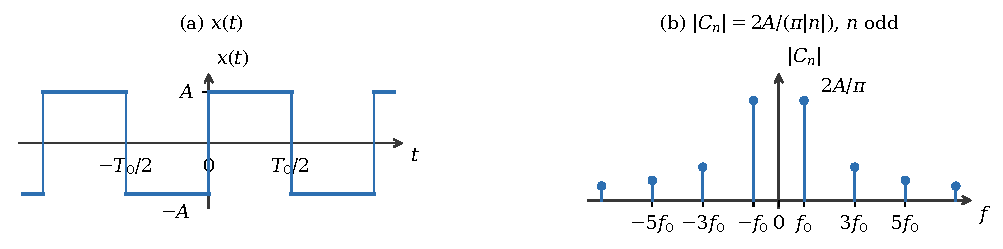
\includegraphics[width=.98\linewidth]{review-square-wave.pdf}
\end{center}
图示取 $A>0$。右图为双边复指数级数的幅值 $|C_n|$，并非三角形式的单边幅值 $b_n$；偶次谐波与直流分量为零。}

\Needspace{8cm}
\subsection{信号的强度：均值、绝对均值与有效值}
\noindent\keypoint{复习重点：区分不同的平均量，掌握正弦信号的绝对均值与有效值。}

\dfn{一周期内的强度参数}{
\begin{align*}
\mu_x&=\frac{1}{T_0}\int_{t_*}^{t_*+T_0}x(t)\diff t &&\text{均值（直流分量）},\\
\mu_{|x|}&=\frac{1}{T_0}\int_{t_*}^{t_*+T_0}|x(t)|\diff t &&\text{绝对均值（整流平均值）},\\
\psi_x^2&=\frac{1}{T_0}\int_{t_*}^{t_*+T_0}|x(t)|^2\diff t &&\text{均方值},\\
x_{\mathrm{rms}}&=\sqrt{\psi_x^2} &&\text{方均根值（有效值）}.
\end{align*}
峰值通常取 $x_p=\max|x(t)|$，峰峰值为 $x_{p-p}=x_{\max}-x_{\min}$。}

由平均不等式，$|\mu_x|\leq\mu_{|x|}\leq x_{\mathrm{rms}}$。对正弦信号，
\[
\mu_x=0,\quad \mu_{|x|}=\frac{2|x_0|}{\pi},\quad
x_{\mathrm{rms}}=\frac{|x_0|}{\sqrt{2}},\quad x_{p-p}=2|x_0|.
\]

\begin{center}
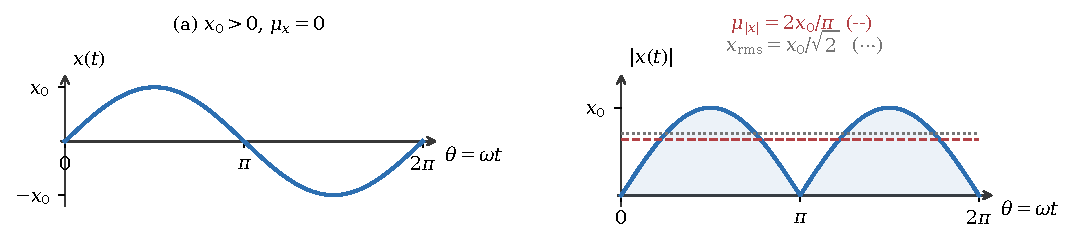
\includegraphics[width=.95\linewidth]{review-sine-strength.pdf}
\end{center}
图示取 $x_0>0$，阴影是一个周期内的整流面积。虚线表示绝对均值；点线表示有效值，它由平方后平均得到，不是整流曲线的平均高度。

\nt{绝对均值 $\mu_{|x|}$ 是信号取绝对值后的平均，不等于均值的绝对值 $|\mu_x|$。求有效值必须先平方、再平均、最后开方。}

\ex{平均功率与谱线强度的联系}{对实周期信号，Parseval关系给出
\[
P_x=x_{\mathrm{rms}}^2=a_0^2+\frac12\sum_{n=1}^{\infty}(a_n^2+b_n^2)
=\sum_{n=-\infty}^{\infty}|C_n|^2.
\]
所以一条三角形式谐波贡献 $A_n^2/2$ 的平均功率，双边复指数的每条线贡献 $|C_n|^2$。此关系用于复习时核对有效值。}

\Needspace{9cm}
\section{瞬变非周期信号与连续频谱}

\subsection{变换约定、频谱密度与画图方法}

\dfn{傅里叶变换对}{使用频率 $f$（单位Hz）时，变换与逆变换为：
\[
X(f)=\mathcal{F}\{x(t)\}=\int_{-\infty}^{\infty}x(t)e^{-\iu2\pi ft}\diff t,
\qquad
x(t)=\int_{-\infty}^{\infty}X(f)e^{\iu2\pi ft}\diff f.
\]
角频率版本记作 $\widetilde X(\Omega)$：
\[
\widetilde X(\Omega)=\int x(t)e^{-\iu\Omega t}\diff t,
\qquad
x(t)=\frac{1}{2\pi}\int \widetilde X(\Omega)e^{\iu\Omega t}\diff\Omega.
\]
两者满足 $X(f)=\widetilde X(2\pi f)$。变量代换遇到冲激时还要使用 $\delta(kz)=\delta(z)/|k|$。}

将周期延长至无穷时，谱线间隔 $1/T_0$ 趋于零，离散谱过渡为连续的\textbf{频谱密度}。若 $x(t)$ 的单位为某物理量，$X(f)$ 的单位为该物理量乘秒；它与傅里叶级数系数 $C_n$ 的单位不同。

\[
X(f)=X_R(f)+\iu X_I(f)=|X(f)|e^{\iu\phi(f)},
\]
\[
|X(f)|=\sqrt{X_R^2(f)+X_I^2(f)},\qquad
\phi(f)=\operatorname{atan2}\bigl(X_I(f),X_R(f)\bigr).
\]
\textbf{幅频图}画模，\textbf{相频图}画相位；\textbf{实频谱与虚频谱}分别画 $X_R$、$X_I$。对实信号，$X(-f)=X^*(f)$，故模是偶函数，相位在模 $2\pi$ 的意义下为奇对称。

\begin{focusbox}{频谱作图的检查顺序}
先标横坐标 $f$ 及单位；再判对称性、求 $f=0$ 值、找峰和零点、看高频趋势；最后算相位并标出无定义点。若谱为实函数，正值处相位为0，负值处为 $\pi$（或 $-\pi$），零点处无定义。画冲激谱时用箭头标注\textbf{权重/面积}，不要当成有限高度曲线。
\end{focusbox}

\Needspace{7cm}
\subsection{线性、尺度、时移、频移与对称性}

\thm{常用变换性质}{设 $x(t)\leftrightarrow X(f)$，$y(t)\leftrightarrow Y(f)$，则
\begin{align*}
\alpha x(t)+\beta y(t)&\leftrightarrow\alpha X(f)+\beta Y(f),\\
x(kt)&\leftrightarrow\frac{1}{|k|}X\left(\frac{f}{k}\right),\quad k\ne0,\\
x(t-t_0)&\leftrightarrow X(f)e^{-\iu2\pi ft_0},\\
x(t)e^{\iu2\pi f_ct}&\leftrightarrow X(f-f_c),\\
x(-t)&\leftrightarrow X(-f),\qquad x^*(t)\leftrightarrow X^*(-f),\\
X(t)&\leftrightarrow x(-f)\quad\text{（对偶性，采用Hz约定）}.
\end{align*}}

\begin{itemize}
\item 时间压缩 $|k|>1$ 会使频谱展宽，幅值密度缩小至 $1/|k|$；时间伸展则相反。
\item 时移改变相位而不改变幅频谱；向右延迟 $t_0$ 对应相位增加 $-2\pi ft_0$。
\item 乘 $e^{\iu2\pi f_ct}$ 使频谱向右搬移 $f_c$。记忆“时域指数正号，频域括号减号”。
\end{itemize}

\begin{table}[H]
\centering
\begin{tabular}{@{}ll@{}}
\toprule
时域类型 & 频域类型 \\
\midrule
实偶函数 & 实偶函数 \\
实奇函数 & 纯虚奇函数 \\
纯虚偶函数 & 纯虚偶函数 \\
纯虚奇函数 & 实奇函数 \\
\bottomrule
\end{tabular}
\end{table}

\nt{采用常规虚部定义时，
\[
X_R(f)=\int x(t)\cos(2\pi ft)\diff t,\qquad
X_I(f)=-\int x(t)\sin(2\pi ft)\diff t
\]
（上式针对实 $x(t)$）。负号来自变换核，不可遗漏。实信号的实部偶、虚部奇，并不意味着频谱整体一定为实数。}

\Needspace{5cm}
\subsection{卷积、加窗与正余弦调制}
\noindent\keypoint{复习重点：用频移和卷积解释截断、衰减振荡与余弦调制的频谱。}

\dfn{时域卷积}{
\[
(x*y)(t)=\int_{-\infty}^{\infty}x(\tau)y(t-\tau)\diff\tau.
\]
卷积中的 $*$ 表示运算，共轭中的上标 $^*$ 表示复共轭，两者含义不同。}

\thm{卷积与乘积对应关系}{
\[
x(t)*y(t)\leftrightarrow X(f)Y(f),\qquad
x(t)y(t)\leftrightarrow(X*Y)(f).
\]
欧拉公式与频移性质进一步给出
\begin{align*}
x(t)\cos(2\pi f_ct)&\leftrightarrow\frac12\bigl[X(f-f_c)+X(f+f_c)\bigr],\\
x(t)\sin(2\pi f_ct)&\leftrightarrow\frac{1}{2\iu}\bigl[X(f-f_c)-X(f+f_c)\bigr].
\end{align*}}

\textbf{加窗：}记录有限时长的数据，相当于将原信号与窗 $w(t)$ 相乘，频域为 $X*W$。理想谱线被窗谱展宽为主瓣及旁瓣，出现频谱泄漏。延长记录使矩形窗主瓣更窄，但不能完全消除旁瓣。

\textbf{调制：}乘以余弦后得到正、负载频处各一份频谱，\textbf{每份系数均为 $1/2$}。相位和复数叠加必须在求模之前完成；一般 $|X_1+X_2|\ne|X_1|+|X_2|$。

\Needspace{8cm}
\subsection{微分、积分与零频项}
\noindent\keypoint{复习重点：微分会消去直流分量，积分频谱需正确处理零频冲激项。}

\thm{微分与积分性质}{在适用的经典或广义变换意义下，
\[
\frac{\diff^n x}{\diff t^n}\leftrightarrow(\iu2\pi f)^nX(f),\qquad
(-\iu2\pi t)^nx(t)\leftrightarrow\frac{\diff^nX}{\diff f^n}.
\]
对 $y(t)=\int_{-\infty}^{t}x(\tau)\diff\tau$，当 $x$ 的变换在零频附近足够规则时，
\[
Y(f)=\PV\!\left(\frac{X(f)}{\iu2\pi f}\right)+\frac{X(0)}{2}\delta(f).
\]
若 $X(0)=0$，零频冲激项消失。一般情形不能仅写“除以 $\iu2\pi f$”。}

\nt{从 $y'(t)=x(t)$ 只能推出 $\iu2\pi fY(f)=X(f)$，无法确定直流冲激项，因为 $f\delta(f)=0$。这正是求阶跃频谱时必须保留 $\tfrac12\delta(f)$ 的原因。$\PV$ 表示主值分布；本章只需理解其在 $f=0$ 附近不能当普通函数积分。}

\clearpage
\subsection{矩形窗、冲激、常量与正余弦变换对}

\dfn{矩形窗与Sa函数}{为避免两种sinc约定混淆，记
\[
\Sa(z)=\begin{cases}\sin z/z,&z\ne0,\\1,&z=0.\end{cases}
\]
若窗的\textbf{总宽度为 $L$}，则
\[
w_L(t)=\begin{cases}1,&|t|<L/2,\\0,&|t|>L/2,\end{cases}
\quad\leftrightarrow\quad W_L(f)=L\Sa(\pi Lf).
\]
若窗区间为 $[-T,T]$，总窗宽便是 $L=2T$，相应 $W(f)=2T\Sa(2\pi Tf)$。}

\begin{center}
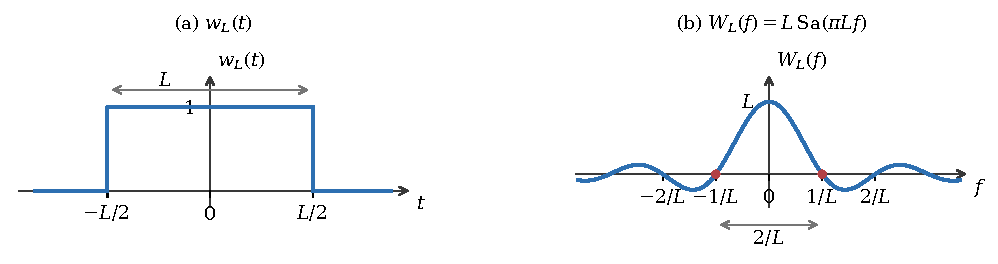
\includegraphics[width=.95\linewidth]{review-rectangular-window.pdf}
\end{center}
左图标出\textbf{总窗宽 $L$}；右图保留窗谱的正、负旁瓣，幅频图应另取绝对值。首零点为 $\pm1/L$，两者间距为主瓣宽 $2/L$。

矩形窗谱为实偶函数，$W_L(0)=L$；零点为 $f=n/L$（非零整数 $n$），零点间的中央主瓣宽 $2/L$。$\Sa$ 的分子正弦是周期函数，但 $\Sa$ 本身是非周期的衰减振荡。若采用归一化 $\operatorname{sinc}(z)=\sin(\pi z)/(\pi z)$，则 $W_L(f)=L\operatorname{sinc}(Lf)$。

\dfn{冲激及取样、卷积性质}{冲激 $\delta$ 是广义函数，其含义由积分定义：
\[
\int_{-\infty}^{\infty}\delta(t-t_0)g(t)\diff t=g(t_0).
\]
因此 $\delta(t+t_0)$ 取出 $g(-t_0)$。此外，
\[
x(t)*\delta(t-t_0)=x(t-t_0),\qquad
\delta(kt)=\frac{1}{|k|}\delta(t),\quad k\ne0.
\]}

\Needspace{5cm}
\begin{Theorem}[breakable=false]{基本广义变换对}{}
\begin{align*}
\delta(t)&\leftrightarrow1,& 1&\leftrightarrow\delta(f),\\
\delta(t-t_0)&\leftrightarrow e^{-\iu2\pi ft_0},&
e^{\iu2\pi f_0t}&\leftrightarrow\delta(f-f_0),\\
\cos(2\pi f_0t)&\leftrightarrow\tfrac12[\delta(f-f_0)+\delta(f+f_0)],\\
\sin(2\pi f_0t)&\leftrightarrow\tfrac{1}{2\iu}[\delta(f-f_0)-\delta(f+f_0)].
\end{align*}
\end{Theorem}

对周期信号 $x(t)=\sum_nC_ne^{\iu2\pi nf_0t}$，相应广义傅里叶变换为
\[
X(f)=\sum_{n=-\infty}^{\infty}C_n\delta(f-nf_0).
\]
傅里叶级数给出谱线系数；傅里叶变换把这些系数记为冲激权重。对不绝对可积的常量、正弦、阶跃等信号，不能强行按普通收敛积分处理。

\Needspace{8cm}
\section{周期脉冲序列与采样}

\dfn{周期单位脉冲序列}{采样周期 $T_s>0$、采样频率 $f_s=1/T_s$，定义
\[
p_{T_s}(t)=\sum_{n=-\infty}^{\infty}\delta(t-nT_s).
\]
一个周期内冲激面积为1，故所有傅里叶级数系数都为 $1/T_s$，其频谱为
\[
P_{T_s}(f)=\frac{1}{T_s}\sum_{k=-\infty}^{\infty}\delta(f-kf_s).
\]}

\subsection{时间采样对应频谱周期复制}

将连续信号乘以脉冲序列，得到理想采样信号
\[
x_s(t)=x(t)p_{T_s}(t)=\sum_nx(nT_s)\delta(t-nT_s).
\]
运用时域乘积、频域卷积和冲激移位，
\[
X_s(f)=X(f)*P_{T_s}(f)=\frac{1}{T_s}\sum_kX(f-kf_s).
\]
即频谱以 $f_s$ 为间隔周期复制，每份带有 $1/T_s$ 因子。采样后的脉冲加权信号 $x_s(t)$ 与样本序列 $x[n]=x(nT_s)$ 是相关但不同的数学对象。

若 $X(f)=0$ 于 $|f|>f_m$，使相邻复制频带分离的充分条件为
\[
f_s>2f_m.
\]
实际采样应留出过渡带。若复制谱重叠，会产生混叠，通常无法仅通过理想低通滤波恢复原频谱。采样与余弦调制都可以通过频带端点判断重叠：余弦调制产生两份搬移谱，采样则产生\textbf{无限多份}周期复制谱。

\subsection{频率采样对应时间周期延拓}

若在频域以间隔 $\Delta f$ 取样，
\[
X_d(f)=X(f)\sum_k\delta(f-k\Delta f),
\]
对偶性给出时域的周期复制
\[
x_d(t)=\frac{1}{\Delta f}\sum_nx\left(t-\frac{n}{\Delta f}\right).
\]
因此时间周期为 $1/\Delta f$。这体现“一个域离散化，另一个域周期化”，归一化系数须结合脉冲序列定义核对。

\Needspace{6cm}
\section{随机信号的基本概念}

随机信号的单次波形不能事先准确预测，需要用概率统计方法描述。在相同条件下重复观测，可得到不同的样本函数；这些样本函数共同构成一个随机过程。均值描述平均水平，方差描述围绕均值的波动程度。

平稳性描述统计特征与时间平移的关系。严格平稳过程的有限维概率分布在时间平移下保持不变；广义平稳过程要求二阶矩有限，均值不随时间变化，且自相关只取决于时间间隔。非平稳信号的统计特征会随时间变化，例如噪声强度随工况改变。

\nt{随机信号的某次观测值可以不断变化，而统计特征仍保持稳定。“平稳”指统计规律稳定，不是波形保持不变；仅观察一次波形，也不能充分判定一个随机过程是否平稳。}
